\documentclass[11pt]{article}
\usepackage{physics,slashed}
% NOTE: Add in the relevant information to the commands below; or, if you'll be using the same information frequently, add these commands at the top of paolo-pset.tex file. 
\newcommand{\name}{TA: Hossein Mohammadi}
\newcommand{\email}{hossein.mohammadi.00427@gmail.com}
\newcommand{\classnum}{Advanced Quantum Field Theory}
\newcommand{\subject}{Subject: Effective Action and Its Relation to $W[J]$}
\newcommand{\instructors}{Dr. Amin Faraji}
\newcommand{\assignment}{PSet 4}
\newcommand{\semester}{- Fall 1402}
\newcommand{\duedate}{dd/mm/yyyy}

\input{paolo-pset.tex}

% NOTE: To compile a version of this pset without problems, solutions, or reflections, uncomment the relevant line below.

%\excludeversion{problem}
%\excludeversion{solution}
%\excludeversion{reflection}

\begin{document}	
	
	% Use the \psetheader command at the beginning of a pset. 
	\psetheader
	
	\section*{Problem 1: Effective Action Rudiments}
	
	\begin{problem}
		The idea of effective action is to replace the full quantum theory with a classical action $\Gamma[\phi]$, which carries the same data about the amplitudes essentially. Since quantum theories deviate from classical counterparts at loops, the classical theory $\Gamma[\phi]$ should encode all loops in its tree-level
		
		For example, QED's effective action is:
		\[
		\Gamma_{QED}= \int d^4x \; \Big[
		\bar{\psi} \big(i\slashed{\partial}-m + \Sigma(i\slashed{\partial})\big)\psi 
		-e\bar{\psi} \Gamma^\mu (i\slashed{\partial})A_\mu \psi
		-\frac12 A_\mu \big(
		\partial^\mu\partial^\nu - \Box \eta^{\mu\nu}
		\big)\big(
		1-\Pi(-\Box)
		\big)
		A_\nu + \dots
		\Big]
		\]
		
		\noindent
		Where $\Sigma(\slashed{p})$, $\Gamma^\mu(\slashed{p})$, and $\Pi(p^2)$ are 1PI graphs contributing to electron self-energy, vertex correction, and vacuum polarization respectively. Don't worry about this Lagrangian and vague expressions; you'll see them later.
	\end{problem}
	\begin{enumerate}
		\item
		\begin{problem}{\points{-}}
			\textbf{1PI Diagrams:}
			
			\noindent
			Draw the first few 1PI diagrams contributing to $\Sigma(\slashed{p})$, $\Gamma^\mu(\slashed{p})$, and $\Pi(p^2)$. More specifically, complete the diagrams below by adding suitable components. Also, mention the order in perturbation theory.
			
			\begin{figure}[H]
				\centering
				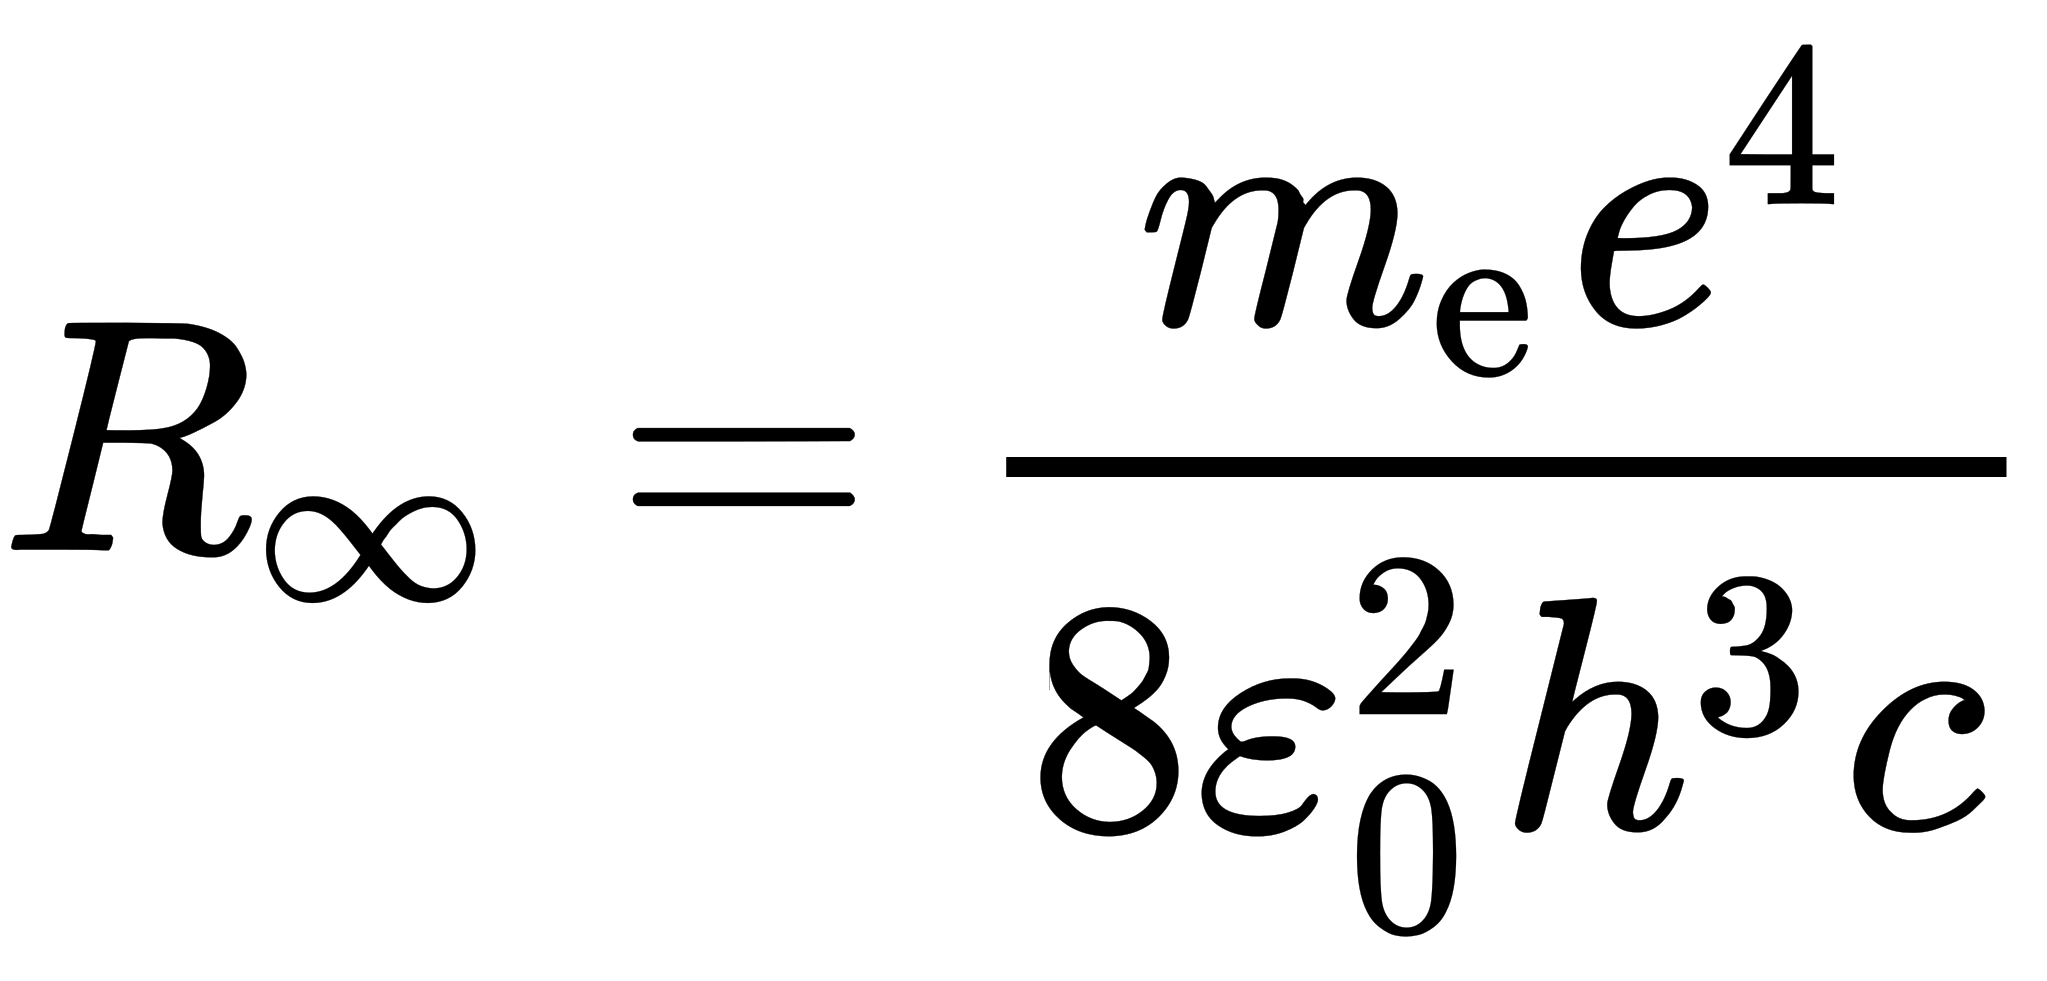
\includegraphics[width=0.5\linewidth]{img/1.png}
				\caption{1PI contributions to QED Lagrangian.}
			\end{figure}
		\end{problem}
	
		\item
		\begin{problem}{\points{-}}
		\textbf{$W[J]$ and its interpretation}
		
	As you know, $\Gamma[\phi]$ is the Legendre transformation of the generating functional of connected diagrams, $W[J]$. In this part of the problem, we want to establish their equivalence.
	
	\begin{enumerate}
		\item To begin with, let's check if $W[J]$ generates connected diagrams.
		\[
		(-i\hbar)^n \frac{\partial^n W[J]}{\partial J(x_1)\dots \partial J(x_n)} = -i\hbar \bra{J} T{\phi(x_1) \dots \phi(x_m)}\ket{J}_{Connected}
		\]
		
		For $n=2,3$, show that it, indeed, generates connected Feynman diagrams. (Just plug back $W[J] = -i\hbar \ln(Z[J])$ into the above relation and take the derivatives.)
		
		For general $n$, argue that the expression gives the connected n-point functions.
	\end{enumerate}
	
		\end{problem}
	\item
	\begin{problem}{\points{-}}
		\textbf{The relation between $\Gamma[\phi]$ and $W[J]$}
		
		\noindent
		The ultimate result is that 
		\[
		\Gamma[\phi] = W[J_\phi] - \int d^4x \; J_\phi(x) \phi(x)
		\]
		Where $J_\phi(x)$ is an implicit functional, $\frac{\partial W[J]}{\partial J(x)}\Big|_{J=J_{\phi}} = \phi(x) $.
		
		Compute $\frac{\partial \Gamma[\phi]}{\partial \phi(x)}$ by chain rule and define the inverse transformation.
	\end{problem}

	\item
\begin{problem}{\points[\textbf{Optional, just read it.}]{-}}
	\textbf{How is this possible?}
	
	\noindent
	You may ask why effective action has such a simple relation with $W[J]$? Here's a simple proof.
	
	As you know, all connected diagrams can be found either by $W[J]$ or by classical action, which is $\Gamma[\phi]$. In the path integral, classical stuff means take $\hbar \xrightarrow{} 0$ limit.
	\[
	W[J] \equiv \lim_{\hbar \to 0} (-i\hbar) \ln \Big(
	\int \mathcal{D}\phi \exp{\frac{i}{\hbar} \big(\Gamma[\phi] + \int d^4x J(x)\phi(x)\big)}
	\Big)
	\]
	Taking this limit means that only classical field (that exteremizes the exponential) will survive. The exteremum occurs at
	\[
	\phi_J = \frac{\partial \Gamma}{\partial \phi}\Big|_{\phi = \phi_J} = -J
	\] 
	By substituting back into the above relation:
	\[
	W[J] = \Gamma[\phi_J] + \int d^4x J(x)\phi_J(x)
	\]
	Seems familiar.
\end{problem}

\item
\begin{problem}{\points{-}}
	\textbf{Check the free theory}
	
	Let's check this formal procedure on $\mathscr{L} = -\frac12 \phi (\Box + m^2) \phi$
	
	\noindent
	\begin{enumerate}
		\item Calculate $W[J]$.
		\item Find $J_\phi$.
		\item Find $\Gamma[\phi]$. Express the moral lesson you've got from this exercise. (Hint: What's the relation between quantum action and effective action of a free theory?)
		\item Show that $\Gamma[\phi]$ is minimized by $<\!\!\phi\!\!>$, which is the expectation value of the field operator on the vacuum $\ket{0}$.
	\end{enumerate}
\end{problem}
\end{enumerate}
\textbf{Aside:} As I told earlier, I prefer not to explore advanced stuff like Yang-Mills and their quantization. Although it's the true playground for both the Faddeev-Popov procedure and BRST symmetry, it's better not to open up a new topic\footnote{One can utilize these to quantize string theory. We can talk about it if you would like to.}. Soon, when we start renormalization, you'll be bombarded with different exercises and calculations. So it's fair to have a rest for now.











\end{document}